\documentclass{article}

\usepackage{fancyhdr}
\usepackage{extramarks}
\usepackage{amsmath}
\usepackage{hyperref}
\usepackage{amsthm}
\usepackage{amsfonts}
\usepackage{tikz}
\usepackage[plain]{algorithm}
\usepackage{algpseudocode}
\usepackage{graphicx}
\usetikzlibrary{automata,positioning}
\usepackage{listings}

%
% Basic Document Settings
%

\topmargin=-0.45in
\evensidemargin=0in
\oddsidemargin=0in
\textwidth=6.5in
\textheight=9.0in
\headsep=0.25in

\linespread{1.1}

\pagestyle{fancy}
\lhead{\hmwkAuthorName}
\chead{\hmwkClass\ : \hmwkTitle}
\rhead{\firstxmark}
\lfoot{\lastxmark}
\cfoot{\thepage}

\renewcommand\headrulewidth{0.4pt}
\renewcommand\footrulewidth{0.4pt}

\setlength\parindent{0pt}

%
% Create Problem Sections
%

\newcommand{\enterProblemHeader}[1]{
    \nobreak\extramarks{}{Problem \arabic{#1} continued on next page\ldots}\nobreak{}
    \nobreak\extramarks{Problem \arabic{#1} (continued)}{Problem \arabic{#1} continued on next page\ldots}\nobreak{}
}

\newcommand{\exitProblemHeader}[1]{
    \nobreak\extramarks{Problem \arabic{#1} (continued)}{Problem \arabic{#1} continued on next page\ldots}\nobreak{}
    \stepcounter{#1}
    \nobreak\extramarks{Problem \arabic{#1}}{}\nobreak{}
}

\setcounter{secnumdepth}{0}
\newcounter{partCounter}
\newcounter{homeworkProblemCounter}
\setcounter{homeworkProblemCounter}{1}
\nobreak\extramarks{Problem \arabic{homeworkProblemCounter}}{}\nobreak{}

%
% Homework Problem Environment
%
% This environment takes an optional argument. When given, it will adjust the
% problem counter. This is useful for when the problems given for your
% assignment aren't sequential. See the last 3 problems of this template for an
% example.
%
\newenvironment{homeworkProblem}[1][-1]{
    \ifnum#1>0
        \setcounter{homeworkProblemCounter}{#1}
    \fi
    \section{Problem \arabic{homeworkProblemCounter}}
    \setcounter{partCounter}{1}
    \enterProblemHeader{homeworkProblemCounter}
}{
    \exitProblemHeader{homeworkProblemCounter}
}

%
% Homework Details
%   - Title
%   - Due date
%   - Class
%   - Section/Time
%   - Instructor
%   - Author
%

\newcommand{\hmwkTitle}{Homework\ \#4 (1 Day  Late, 5/5 total) }
\newcommand{\hmwkDueDate}{May 4, 2018}
\newcommand{\hmwkClass}{BMI 776}
\newcommand{\hmwkClassTime}{}
\newcommand{\hmwkClassInstructor}{}
\newcommand{\hmwkAuthorName}{\textbf{John Steill}}


%
% Title Page
%

\title{
    \vspace{2in}
    \textmd{\textbf{\hmwkClass:\ \hmwkTitle}}\\
    \normalsize\vspace{0.1in}\small{Due\ on\ \hmwkDueDate\ at 3:10pm}\\
    \vspace{0.1in}\large{\textit{\hmwkClassInstructor\ \hmwkClassTime}}
    \vspace{3in}
}

\author{\hmwkAuthorName}
\date{}

\renewcommand{\part}[1]{\textbf{\large Part \Alph{partCounter}}\stepcounter{partCounter}\\ }

%
% Various Helper Commands
%

% Useful for algorithms
\newcommand{\alg}[1]{\textsc{\bfseries \footnotesize #1}}

% For derivatives
\newcommand{\deriv}[1]{\frac{\mathrm{d}}{\mathrm{d}x} (#1)}

% For partial derivatives
\newcommand{\pderiv}[2]{\frac{\partial}{\partial #1} (#2)}

% Integral dx
\newcommand{\dx}{\mathrm{d}x}

% Alias for the Solution section header
\newcommand{\solution}{\textbf{\large Solution}}

% Probability commands: Expectation, Variance, Covariance, Bias
\newcommand{\E}{\mathrm{E}}
\newcommand{\Var}{\mathrm{Var}}
\newcommand{\Cov}{\mathrm{Cov}}
\newcommand{\Bias}{\mathrm{Bias}}

\begin{document}

%\maketitle

\pagebreak

\begin{homeworkProblem}
\textbf{1A: Generating simplified theoretical spectra: spectra\_generator.py}

 \vspace{3 mm}
 
\textbf{1B: Computing cross-correlation scores: xcorr.py}
\end{homeworkProblem}

\begin{homeworkProblem}
\textbf{2A: Source-target paths in networks: Complete the implementation of find\_paths.py}
\vspace{3 mm}
 
\textbf{2B: Test your implementation on a new network}
\vspace{3 mm}
 
\textbf{2C: Compare min cost flow and shortest paths}

\begin{figure}[H]
  \centering
  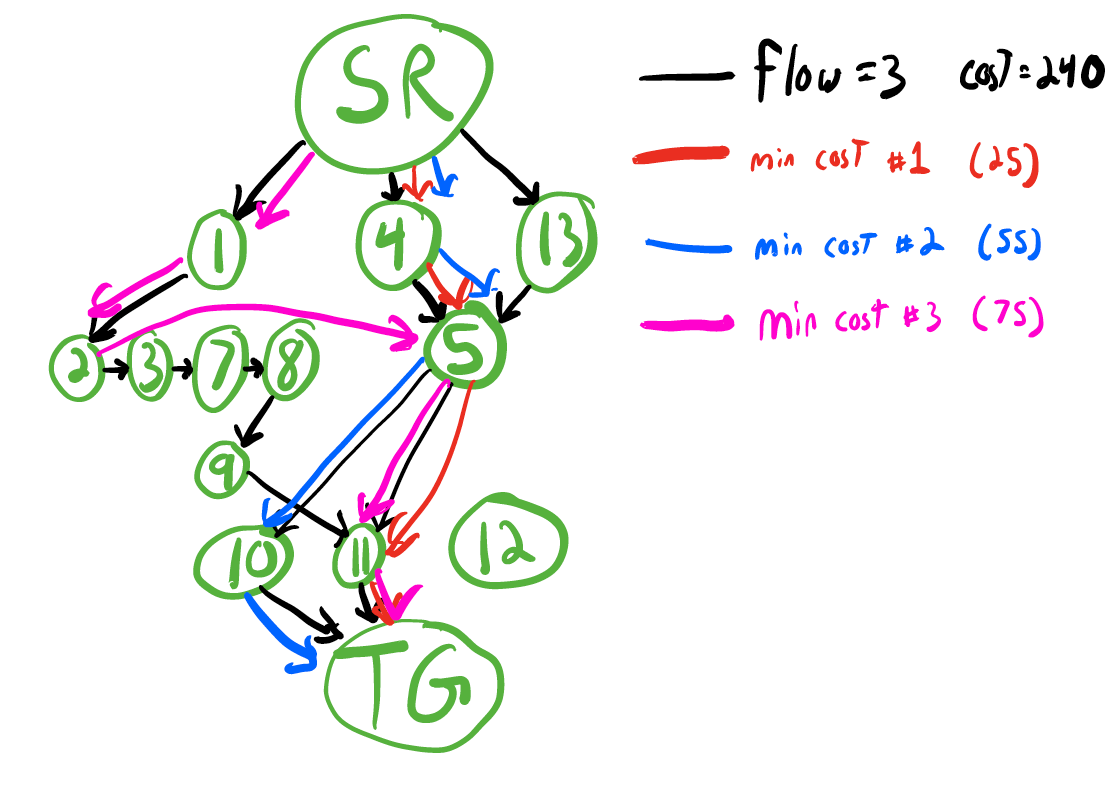
\includegraphics[width=6in]{P2_Sketch.png}
  \caption{Flow = 3 solution vs 3 minimum cost paths}
\end{figure}
 
 We note the optimal solution cost for flow=3 units is 240, with is greater than the sum of the three most optimal paths, which is 155. This is because the superposition of the three paths is not itself a feasible solution. It would demand a capacity in the 5-11 edge of 2, and we are given it to be 1.  More generally, it could be the case where using a lower cost path precludes the use of several other slightly worse paths and forces the use of a very costly path. This local maxima behavior is eliminated by using linear programming algorithms.
 
\vspace{3 mm}

To contrast the advantages of each method, remember the motivation of our problem, to generate useful hypothesis of how information from a cell wall results in change in gene expression levels.
\begin {itemize}
	\item{A min-cost flow solution will help us choose between competing networks in generating the most likely candidate pathways.}
	\item{Examining min-cost paths individually will help us in discovering pathway boundaries and discovering novel pathways.}
\end{itemize}
 

\vspace{3 mm}
\textbf{2D: Special cases of the algorithms}

To assure that the optimal flow solution is the same as superposition of the k shortest paths, we need to assure:
\begin {itemize}
	\item{The superposition of solutions is not infeasible}
	\item{The capacities are sufficiently small to force all k paths to be used.}
\end{itemize}

A sufficient algorithm:
\begin {itemize}
	\item{Choose f and k}
	\item{Count all source edges in k, set each edge capacity to the multiple of $\frac{f}{|edges|}$ proportional to its count.}
	\item{For all other edges: with nodes \textit{in} and \textit{out}, set capacity to $\frac{\text{inflow to in}}{\text{count of edges from out in k paths}}$ }
\end{itemize}

For our problem, for existing capacities, only the flow = 1 and k = 1 solutions are the same. If we increase capacities to 2, then the flow = 3 and k = 3 superpositions are the same. 

\end{homeworkProblem}

\newpage

\begin{homeworkProblem}
\textbf{3A: Interpolated Markov models: $\chi^2$ test}

\vspace{3 mm}

\begin{tabular}{|| c | c c c ||} 
\hline
Seq & $C_4$ & $C_3$ & $C_2$\\
\hline
TTAA & 15 & 85 & 450 \\
TTAC & 20 & 70 & 220 \\ 
TTAG & 10 & 35 & 180 \\ 
TTAT & 5 & 10 & 50 \\
\hline
& 50 & 200 & 900 \\
\hline
\end{tabular} 

\vspace{3 mm}

\textbf{3A.i : $\chi^2_{3,2}$}

\begin{align*}  
E_{1,1} &= \frac{100 * 50}{250} = 20 &  E_{1,2} = \frac{100 * 200}{250} =80 \\
E_{2,1} &= \frac{90 * 50}{250} = 18 &  E_{2,2} = \frac{90 * 200}{250} = 72 \\
E_{3,1} &= \frac{45 * 50}{250} = 9 &  E_{1,2} = \frac{45 * 200}{250} =36 \\
E_{4,1} &= \frac{15 * 50}{250} = 3 &  E_{2,2} = \frac{15 * 200}{250} = 12 \\
\end{align*} 

\begin{eqnarray*}  
\chi^2_{3,2} & = & \sum_{m=1}^2\sum_{k=1}^4\frac{(E_{m,k}-O_{m,k})^2}{E_{m,k}}\\
 & = & \frac{(15-20)^2}{20} + \frac{(20-18)^2}{18} + \frac{(10-9)^2}{9}\ + \frac{(5-3)^2}{3}\\
 & + &  \frac{(85-80)^2}{80} + \frac{(70-72)^2}{72} + \frac{(35-36)^2}{36}\ + \frac{(10-12)^2}{12}\\
 & = & 1.25  + 0.222 +  0.111 +  1.333 + .3125 + .0556 + .0278 + .3333  \\
 & = & 3.646 \\
\end{eqnarray*}  

\begin{eqnarray*} 
p &=& 0.308022171558994 + \frac{3.646 -3.6}{3.7-3.6}(0.295734032375276 - 0.308022171558994) \\
&=&0.3023942038128512 \approx 0.302\\
d &=& 1-p = 0.698
\end{eqnarray*} 

\textbf{3A.ii : $\chi^2_{2,1}$}

\begin{align*}  
E_{1,1} &= \frac{535 * 200}{1100} = 97.27 &  E_{1,2} = \frac{535 * 900}{1100} =437.73 \\
E_{2,1} &= \frac{290 * 200}{1100} = 52.73 &  E_{2,2} = \frac{290 * 900}{1100} = 237.27 \\
E_{3,1} &= \frac{215 * 200}{1100} = 39.09 &  E_{1,2} = \frac{215 * 900}{1100} = 175.91 \\
E_{4,1} &= \frac{60 * 200}{1100} = 10.91 &  E_{2,2} = \frac{60 * 900}{1100} = 49.09 \\
\end{align*} 


\begin{eqnarray*}  
\chi^2_{2,1} & = & \sum_{m=1}^2\sum_{k=1}^4\frac{(E_{m,k}-O_{m,k})^2}{E_{m,k}}\\
 & = & 1.548 + 5.658 + 0.4281 + 0.0758 + 0.3441 + 1.2574 + 0.0951 + 0.0168\\
 & = & 9.4240 \\
\end{eqnarray*}  

\begin{eqnarray*} 
p &=& 0.0244193373957173 + \frac{9.424-9.4}{9.5-9.4}(0.0233313604308315 - 0.0244193373957173) \\
&=&0.024158222924144705 \approx 0.024\\
d &=& 1-p = 0.976
\end{eqnarray*} 
 
\vspace{3 mm}
\textbf{3B: Calclating $\lambda$ }
\begin{align*}  
\lambda_3 &=d \frac{c}{400} = .698 \frac{50}{400} = 0.0872 \\
\lambda_2 &=d \frac{c}{400} = .976 \frac{200}{400} = 0.488 \\
\lambda_1 &=1 \text{(c greater than 400)} \\
\end{align*} 

\vspace{3 mm}
\textbf{3C: Interpolated Markov model probability}
\begin{align*}  
P_{IMM,1}(A|A) &=  \lambda_1(A)P(A|A) + (1-  \lambda_1(A)) P_{IMM,0}(A)\\
&= 1 * .5 + 0 * P_{IMM,0}(A) = .500 \\
& \\
P_{IMM,2}(A|TA) &=  \lambda_2(TA)P(A|TA) + (1-  \lambda_2(TA)) P_{IMM,1}(A|A)\\
&= .488 * .425 + .512 * .5 = 0.463\\
& \\
P_{IMM,3}(A|TTA) &=  \lambda_3(TTA)P(A|TTA) + (1-  \lambda_3(TTA)) P_{IMM,2}(A|TA)\\
&= .0872 * .3 + .913 * 0.4634 = 0.449\\
\end{align*} 
\end{homeworkProblem}
\end{document}
